% 本章节介绍Qemu的原理
\section{Qemu \& KVM 基本原理}
\subsection{虚拟化}
在维基百科中虚拟化的解释为:“In computing,virtualization refers to the act of creating a virtual(rather than actual)version of something,including virtual computer hardware platforms,storage devices,and computer network resources。”\cite{Wikipedia_Virtualization}, 
简单来说,计算机模拟出一个虚拟并不存在的(而非实际)计算机实体就是虚拟化,其中包括虚拟出来的计算机硬件平台、存储设备,以及网络资源。
由此可见,虚拟化技术是一种将硬件资源(如处理器、Memory、storage、NetWork resource etc)提取出来,最终成为一个虚拟的资源池,并对其提供分割、重新组合的操作,以达到资源利用最大化。

\subsubsection{软件虚拟化}
本文所介绍的是使用Qemu来实现VMM层,即仅使用软件实现的方式来运行客户机要执行的指令。
Qemu工作方式是在软件层面实现对指令的二进制翻译,简单来说就是Qemu是一个翻译官,它将使用某套指令集的二进制编码翻译成基于另一套指令集的编码并最终输出到最终架构下的代码交给客户机,QEMU会拦截每一条客户机执行的指令,并转换成宿主机处理器架构的指令,
最后由宿主机的物理硬件来执行相应的指令,由此往复完成虚拟化的实现。

\subsubsection{硬件虚拟化}
这里以通用的x86体系结构为例,Intel在2005年就加入硬件虚拟化的支持——Intel VT。
这也就以为着硬件平台本身支持客户机与宿主机指令间相互转换并执行,而不再像以前那样需要VMM截获重定向这种软件实现方式。

其实我们通过纯粹用软件中的模块管理层面上直接对管理整个客户机服务的进程就是通过要在整个linux上的一个内部物理执行进程,
客户机正常执行访存操作时,实际上我们就是通过Linux上对内核管理的虚拟内存,以前是使用linux中的内核软件来实现GVA(客户机虚拟地址)到GPA(客户机物理地址)再到HVA(宿主机虚拟地址),最后到HPA(宿主机物理地址)的这四步的转换,这个机制也称为“影子页表”。
但是原本就是访问一个地址很简单的操作却大费周折要经过四步执行,对于计算机来说,这样的代价特别大,所以后来这种靠软件实现的方式逐步被硬件逻辑取代,这种硬件逻辑就是Intel的EPT技术(或者AMD的NPT技术),靠硬件自动算出GPA到HPA的过程,转换的过程一步到位。

\subsection{硬件虚拟化介绍}

\subsubsection{CPU虚拟化}
根据上文的介绍,软件实现虚拟化的成本代价比较大,所以像Intel这样的硬件厂商慢慢地在硬件层面上实现虚拟化。

关键技术——VMX(virtual-machine extensions),
这项技术就是Intel在处理器层面上提供了对实现虚拟化在技术上的支持。
根据查询Intel的官方文档\cite{Intel_VMX}可知 VMX有两种操作模式:VMX根操作(root operation)与VMX非根操作(non-root operation)。

简单的区分,在VMX根操作模式运行KVM下,而VMX非根模式下运行的是整个运行在虚拟机中的客户机完整的软件栈(包括操作系统和应用程序)。VMX根操作模式与非VMX模式之间是可以相互转化的,当从VMX跟模式进入VMX 非根操作模式被称为“VM Entry”;从VMX非根操作模式退出到VMX根操作模式,被称为“VM Exit”。

可能都是Intel发明的缘故,VMX的根操作模式与非VMX模式像极了x86处理器的各种执行模式,
区别只是VMX的根操作现在已经支持了新的VMX相关的指令集以及一些对相关控制寄存器的操作。
而由于VMX的非根操作模式是一个相对受限的执行环境,为了更好地适应在虚拟化中的变化而专门进行了一定的修改;
VMX的根操作模式与非VMX模式之间的转换如同处理器的各种门的特权集转换一样,当客户机中执行的一些特殊的敏感指令或者一些异常会触发“VM Exit”退到虚拟机监控器中,从而运行在VMX根模式。这样的行为看似很麻烦,但是也正是因为这样的限制,才让虚拟机监控器保持了对处理器资源的更好的控制。

为了更好的理解,VMM 与 Guest 之间 以及VMX的根操作模式与非根操作模式是如何转换的,
交互一个虚拟机监控器软件的最基础的运行生命周期及其与客户机的交互如图 \ref{fig:VMM_Guest} 所示。
软件想进入VMM操作模式,需要通过执行VMXON指令才能进入;当已经进入VMM模式以后,想在进入客户机执行模式,即VMX非根模式,需要通过执行VMLAUNCH和VMRESUME指令进入;
当在VMX非根模式下触发VM Exit时,处理器执行控制权会再次回到宿主机的虚拟机监控器上;
最后虚拟机监控可以通过执行VMXOFF指令退出VMX执行模式。

\begin{figure}[htbp]
    \centering
    \def\svgwidth{\columnwidth}
    \import{./figs/RISC-V/KVM/VMM_Guest/}{VMM_Guest.pdf_tex}
    \caption{VMM与Guest之间的交互}
    \label{fig:VMM_Guest}
\end{figure}


如图\ref{fig:VMM_Guest} 中需要完成的转换过程,
在该过程中是通过使用VMCS(virtual-machinecontrol data structure)的数据结构来实现逻辑处理器完成根模式和非根模式之间的切换的;
而处理器是通过使用VMCS指针来进行访问VMCS结构的,并对其进行操作。
其实VMCS指针其实也没什么神奇的,本质上就是一个指向VMCS结构的64位的地址,可以通过使用VMPTRST和VMPTRLD指令对VMCS指针进行读写,使用MREAD、VMWRITE和VMCLEAR等指令对VMCS实现配置。

对于一个逻辑处理器,表面上看它是可以一起维护多个VMCS数据结构,但是具体到某一时刻的时候,就只有一个VMCS在当前真正生效。多个VMCS之间也是可以相互切换的,VMPTRLD指令就让某个VMCS在当前生效,而其他VMCS就自然成为不是当前生效的。一个虚拟机监控器会为一个虚拟客户机上的每一个逻辑处理器维护一个VMCS数据结构。

\subsubsection{内存虚拟化}
内存虚拟化的目的是给虚拟客户机操作系统提供类似实际的物理存储空间——即一个从0地址开始的连续物理内存空间,但是他不仅仅就是提供地址空间,还要同时在多个客户机之间实现隔离和调度。

在虚拟环境下内存地址如图 \ref{fig:Virtual2Physical_Address} 所示。
\begin{figure}[htbp]
    \centering
    \def\svgscale{0.5}
    \import{./figs/RISC-V/KVM/Virtual2Physical_Address/}{Virtual2Physical_Address.pdf_tex}
    \caption{虚拟化环境下的内存地址}
    \label{fig:Virtual2Physical_Address}
\end{figure}

内存虚拟化就是要将客户机虚拟地址(GVA)转化为最终能够访问的宿主机上的物理地址(HPA)。对于客户机操作系统而言,它不可能感知到有内存虚拟化的存在,在应用程序访问虚拟地址时,通过CR3寄存器可以将其转化为物理地址,但是在虚拟化环境中这个物理地址只是客户机的物理地址,还不是真实内存硬件上的物理地址。
所以,虚拟机监控器就非常需要维护从物理客户机虚拟地址映射到客户宿主机上的物理虚拟地址之间的一个动态映射空间关系,
在没有硬件提供的内存虚拟化之前,这个维护映射关系的页表叫作影子页表(Shadow Page Table)。
内存的访问和数据的更新通常是非常频繁的,加之需要一直维护影子页表中的对应关系将会变得非常复杂,开销也较大。同时它还需要为每一个运行的客户机都维护一份影子页表,当客户机数量较多时,其影子页表也会越来越大,占用的内存较大也会是一个问题。

Intel CPU在整个硬件上的设计就引入了EPT(Extended Page Tables,扩展页表),
从而将一个客户机虚拟地址到宿主机物理地址的转换通过硬件来实现。
%首先,通过客户机CR3寄存器将客户机虚拟地址转化为客户机物理地址,然后通过查询EPT来实现客户机物理地址到宿主机物理地址的转化。EPT的控制权在虚拟机监控器中,只有当CPU工作在非根模式时才参与内存地址的转换。使用EPT后,客户机在读写CR3和执行INVLPG指令时不会导致VM Exit,而且客户页表结构自身导致的页故障也不会导致VM Exit。所以通过引入硬件上EPT的支持,简化了内存虚拟化的实现复杂度,同时也提高了内存地址转换的效率。


\subsubsection{I/O虚拟化}
在虚拟化的架构下,虚拟机监控器必须支持来自客户机的I/O请求。通常情况下有以下4种I/O虚拟化方式。

1)设备模拟:在虚拟机监控器中模拟一个传统的I/O设备的特性,比如在QEMU中模拟一个Intel的千兆网卡或者一个IDE硬盘驱动器,在客户机中就暴露为对应的硬件设备。客户机中的I/O请求都由虚拟机监控器捕获并模拟执行后返回给客户机。

2)前后端驱动接口:在虚拟机监控器与客户机之间定义一种全新的适合于虚拟化环境的交互接口,比如常见的virtio协议就是在客户机中暴露为virtio-net、virtio-blk等网络和磁盘设备,在QEMU中实现相应的virtio后端驱动。

3)设备直接分配:将一个物理设备,如一个网卡或硬盘驱动器直接分配给客户机使用,这种情况下I/O请求的链路中很少需要或基本不需要虚拟机监控器的参与,所以性能很好。

4)设备共享分配:其实是设备直接分配方式的一个扩展。在这种模式下,一个(具有特定特性的)物理设备可以支持多个虚拟机功能接口,可以将虚拟功能接口独立地分配给不同的客户机使用。如SR-IOV就是这种方式的一个标准协议。

表\ref{fig:I/O_virtual}展示了这4种I/O虚拟化方式的优缺点,前两种都是纯软件的实现,后两种都需要特定硬件特性的支持。

% 插入表格
\begin{table}[htbp]
     \centering
\begin{tabular}{|c|l|l|}
\hline
\multicolumn{1}{|l|}{} & \textbf{优点}                                                 & \textbf{缺点}                                                                              \\ \hline
设备模拟                   & 兼容性好,不需要额外驱动                                                & \begin{tabular}[c]{@{}l@{}}1.性能较差\\ 2.模拟设备的功能特性支持不够多\end{tabular}                        \\ \hline
前后端接口                  & 性能有所提升                                                      & \begin{tabular}[c]{@{}l@{}}1.兼容性差一些:依赖客户机总安装特定驱动\\ 2.I/O压力大时,后端驱动的CPU资源占用较高\end{tabular} \\ \hline
设备直接分配                 & 性能非常好                                                       & \begin{tabular}[c]{@{}l@{}}1.需要硬件设备的特性支持\\ 2.单个设备只能分配一个客户机\\ 3.很难支持动态迁移\end{tabular}     \\ \hline
设备共享分配                 & \begin{tabular}[c]{@{}l@{}}1.性能非常好\\ 2.单个设备可共享\end{tabular} & \begin{tabular}[c]{@{}l@{}}1.所需设备硬件的特性支持\\ 2.很难支持动态迁移\end{tabular}                       \\ \hline
\end{tabular}
\caption{常见I/O虚拟化方式的优缺点}
\label{fig:I/O_virtual}
\end{table}


\subsection{KVM \& Qemu模拟器介绍}
首先Qemu(Quick Emulator)本身并不完全是KVM的一部分,它是一套由软件模拟实现的。

而KVM(Kernel Virtual Machine)是有两部分组成,一部分是Linux内核的KVM模块,另一块是经过简化后的Qemu。
有了KVM的linux主机将变成一个Hypervisor(虚拟机监控器)。
在x86处理器支持VMX(Virtual Machine Extension)功能以后,
Linux在原有的用户模式和内核模式中又新增加了客户模式,并且客户模式也拥有自己的内核模式和用户模式,其中虚拟机部分就是运行在客户模式中。
三层结构如图\ref{fig:kvm}所示。

\begin{figure}[htbp]
    \centering
    \def\svgscale{0.5}
    \import{./figs/RISC-V/KVM/KVM_3model/}{kvm_3model.pdf_tex}
    \caption{KVM三种模式的层次关系}
    \label{fig:kvm}
\end{figure}    
%『h』当前位置。将图形放置在正文文本中给出该图形环境的地方。如果本页所剩的页面不够,这一参数将不起作用。
%『t』顶部。将图形放置在页面的顶部。
%『b』底部。将图形放置在页面的底部。
%『p』浮动页。将图形放置在一只允许有浮动对象的页面上。

KVM就是在硬件辅助虚拟化技术之上构建起来的虚拟机监控器。

当然,并非要所有这些硬件虚拟化都支持才能运行KVM虚拟化,KVM对硬件最低的依赖是CPU的硬件虚拟化支持。

\subsubsection{KVM内核模块}
KVM模块是KVM虚拟化的核心部分,它在内核是由两部分组成:
其中一个部分是与处理器架构无关的部分,用lsmod命令中可以看到,如图 \ref{fig:lsmod_kvm} 所示,叫作kvm模块;
另一个部分是处理器架构相关的部分,本文是在Intel平台上实验,所以看到的就是 kvm\_intel这个内核模块。
KVM的主要工作就是初始化硬件资源,开启虚拟化模式,将客户机运行在虚拟机模式中,虚拟客户机运行时提供一定的支持。

\begin{figure}[htbp]
  \centering %居中显示
  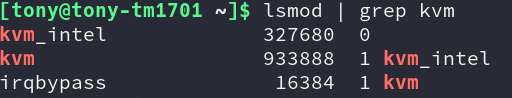
\includegraphics[width=0.9 \textwidth]{figs/RISC-V/KVM/lsmod_kvm.png}
  \caption{lsmod}
  \label{fig:lsmod_kvm} %设置图形引用名称
\end{figure}

以KVM在Intel的x86系列的 CPU上运行为例,在内核加载以后,KVM模块首先会初始化内部的数据结构;
完成一切准备工作以后,KVM模块会继续检测系统当前的CPU,然后打开CPU控制寄存器CR4中的虚拟化模式开关,并通过执行VMXON指令将宿主操作系统(包括KVM模块本身)置于CPU执行模式的虚拟化模式中的根模式;
最后,KVM模块创建特殊设备文件/dev/kvm来等待从用户空间发过来的命令。
接下来,虚拟机的创建和运行将是一个用户空间的应用程序(QEMU)和KVM模块相互配合的过程。

/dev/kvm这个设备文件是一个标准的字符设备,
KVM模块与用户空间QEMU的通信接口主要是一系列针对这个特殊设备文件的loctl调用。
当然,每个虚拟客户机针对/dev/kvm文件的最重要的loctl调用就是“创建虚拟机”。
在这里,“创建虚拟机”可以理解成KVM为了某个特定的虚拟客户机(用户空间程序创建并初始化)创建对应的内核数据结构。同时,KVM还会返回一个文件句柄来代表所创建的虚拟机。针对该文件句柄的loctl调用可以对虚拟机做相应的管理,比如创建用户空间虚拟地址和客户机物理地址及真实内存物理地址的映射关系,再比如创建多个可供运行的虚拟处理器(vCPU)。同样,KVM模块会为每一个创建出来的虚拟处理器生成对应的文件句柄,对虚拟处理器相应的文件句柄进行相应的loctl调用,就可以对虚拟处理器进行管理。

“执行虚拟处理器”是虚拟处理器最重要的loctl调用,通过该调用,可在KVM模块的支持下将用户空间准备好的虚拟客户机放置在虚拟化模式中的非根模式,并执行相应的二进制指令。
在非根模式下执行二进制指令时,如果出现敏感指令会被处理器理科捕捉到,然后保存现场并切换到根模式,接下来的操作就有KVM来决定(一种方法是在KVM模块直接处理,另一种方法是返回到用户空间交让用户空间的程序来进行处理)。

%除了内存处理器的内部虚拟化,内存上的虚拟化也是由kckvm等的模块化来实现的,包括前面我们提到的内存使用虚拟硬件模块提供的kceptm等特性,通过两级内存转换可以实现一个客户机虚拟地址转换到一个宿主机内存物理虚拟地址之间的两级转换。

除了处理器的虚拟化以外,内存虚拟化也是由KVM模块实现的,包括上文中提到的使用硬件提供的EPT特性,通过两次的地址转换机制最终实现从客户机虚拟地址到宿主机物理地址之间的转换。

%处理器对内存设备的数据访问主要方式是通过内存i/o处理指令和内存mmio,其中放在i/o中的指令通常会被内存处理器直接进行截获,mmio指令会通过直接配置放在内存中的虚拟化指令来进行捕捉。但是,外设的功能模拟一般不由k和kvm两个模块自行负责。一般来说,只有对系统性能配置要求比较高的一台虚拟主机设备才可能会由一个kvm内核模块集成来直接对其负责,比如需要虚拟一个中断处理控制器和一个虚拟运行时钟,这样也就可以大量度地减少内核处理器在多模式实时切换的成本开销。而大部分的网络输入输出设备都是交给下一节将要详细介绍的一个用户端状态处理程序例如qemuo##c来进行负责。

处理器主要是通过使用I/O指令和MMIO来实现的对设备的访问,
其中I/O指令是处理器直接截获进行处理,而MMIO会通过配置内存虚拟化来捕捉。
但是,模拟外设的模块一般不是采用KVM模块来负责,因为只有像虚拟中断控制器和虚拟时钟这种对性能要求比较高的虚拟设备才会由KVM内核模块来直接负责,因为这样做可以大量减少因处理器模式来回切换的开销。而大部分的输入输出设备交给下一节将要介绍的用户态程序QEMU来负责。

\subsubsection{QEMU用户态设备模拟}
% qemu原本本身就是一个著名的免费开源网络虚拟机应用软件开发项目,而不是kvmu的虚拟化开发软件的一部分。与qekvm不同,qemu最初需要实现的软件虚拟机功能是一个纯单机软件的虚拟实现,通过使用二进制软件翻译算法来进行实现,而虚拟化是对客户机系统中的q和cpu两个指令集的模拟,所以实际性能比较低。但是,其最大优点仍然是跨平台,qemu支持在solinux、windows、freebsd、solaris、macos等多种不同操作平台系统上同时运行,能直接支持在一个qemu本身是被编译出来运行的一个平台上就可以实现一个虚拟机的运行功能,甚至它还可以直接支持一个客户机与其他宿主机并不是同一个平台架构(比如在 x86平台上运行 ARM客户机)。作为一个已经存在已久的通用虚拟机系统监控器开发软件,qemu的开发代码中可能有完整的一个虚拟机系统实现,包括了微处理器系统虚拟化、内存系统虚拟化,以及qekvm也可能会对使用到的其他虚拟机对设备进行模拟(硬件比如无线网卡、显卡、存储器微控制器和固态硬盘等)。

QEMU原本就是一个著名的开源免费的用于虚拟化的软件项目,并不是KVM软件的一部分。不同于KVM,QEMU最初实现的是一个纯软件的虚拟机,通过使用二进制翻译来实现对虚拟的客户机中CPU指令模拟执行,所以实际性能比较低。
但是,它能发展到今天主要是因为他的一个显著特点——跨平台,QEMU支持在Linux、Windows、FreeBSD、Solaris、MacOS等多种不同的操作系统上运行,能支持在QEMU本身编译运行的平台上就实现虚拟机的功能,甚至可以支持客户机与宿主机并不是同一个架构(比如在x86平台上运行ARM客户机)。
作为一个存在已久的虚拟机监控器软件,QEMU的开发代码中有完整的虚拟机实现,包括处理器虚拟化、内存虚拟化,以及KVM也会用到的虚拟设备模拟(比如网卡、显卡、存储控制器和硬盘等)。

除了二进制翻译的方式,QEMU也能与基于硬件虚拟化的Xen、KVM结合,为它们提供客户机的设备模拟。通过与KVM的密切结合,让虚拟化的性能提升得非常高,在真实的企业级虚拟化场景中发挥重要作用,所以我们通常提及KVM虚拟化时就会说“QEMU/KVM”这样的软件栈。

%最早期的KVM开发者们为了简化软件架构和代码重用,根据KVM特性在QEMU的基础上进行了修改(当然这部分修改已经合并回QEMU的主干代码,故现在的QEMU已原生支持KVM虚拟化特性)。从图2-8可以看出,每一个虚拟客户机在宿主机中就体现为一个QEMU进程,而客户机的每一个虚拟CPU就是一个QEMU线程。虚拟机运行期间,QEMU会通过KVM模块提供的系统调用进入内核,由KVM模块负责将虚拟机置于处理器的特殊模式下运行。遇到虚拟机进行I/O操作时,KVM模块会从上次的系统调用出口处返回QEMU,由QEMU来负责解析和模拟这些设备。

为了简化代码的架构以及让代码复用,KVM的开发者根据KVM的特性在原有的QEMU基础上进行了修改(后来这些代码被合并到QEMU开发主线代码中了,所以现在QEMU已经可以原生支持KVM虚拟了)。虚拟机在运行时,QEMU会通过KVM模块提供的系统调用进入内核,然后KVM模块将其置于处理器的特殊模式下运行。

%从QEMU角度来看,也可以说QEMU使用了KVM模块的虚拟化功能,为自己的虚拟机提供硬件虚拟化的加速,从而极大地提高了虚拟机的性能。除此之外,虚拟机的配置和创建,虚拟机运行依赖的虚拟设备,虚拟机运行时的用户操作环境和交互,以及一些针对虚拟机的特殊技术(如:动态迁移),都是由QEMU自己实现的。

但是站在QEMU的立场而言,QEMU使用了KVM模块的虚拟化功能,来为自身提供硬件虚拟化的加速,从而很大幅度的改进了虚拟机的性能。除此之外,配置和创建虚拟机,虚拟机运行时依赖的虚拟设备、用户交互界面、运行环境,还有一些针对虚拟机的高级技术像动态迁移技术,热备份等等也都是QEMU自身完成实现的。

QEMU除了提供完全模拟的设备(如:e1000网卡、IDE磁盘等)以外,还支持virtio协议的设备模拟。virtio是一个沟通客户机前端设备与宿主机上设备后端模拟的比较高性能的协议,在前端客户机中需要安装相应的virtio-blk、virtio-scsi、virtio-net等驱动,而QEMU就实现了virtio的虚拟化后端。QEMU还提供了叫作virtio-blk-data-plane的一种高性能的块设备I/O方式,它最初在QEMU 1.4版本中被引入。virtio-blk-data-plane与传统virtio-blk相比,它为每个块设备单独分配一个线程用于I/O处理,data-plane线程不需要与原QEMU执行线程同步和竞争锁,而且它使用ioeventfd/irqfd机制,同时利用宿主机Linux上的AIO(异步I/O)来处理客户机的I/O请求,使得块设备I/O效率进一步提高。

总之,QEMU既是一个功能完整的虚拟机监控器,也在QEMU/KVM的软件栈中承担设备模拟的工作。


\subsection{KVM上层管理工具}
虽然本文涉及到的KVM上层管理软件比较少,但是我觉得还是将KVM作为一个完整的整体来处理,这里介绍一下我在阅读KVM官网信息的时候遇到常用的管理工具。

\subsubsection{libvirt}
libvirt是使用最广泛的对KVM虚拟化进行管理的工具和应用程序接口,已经是事实上的虚拟化接口标准,本节后部分介绍的其他工具都是基于libvirt的API来实现的。作为通用的虚拟化API,libvirt不但能管理KVM,还能管理VMware、Hyper-V、Xen、VirtualBox等其他虚拟化方案。

\subsubsection{virsh}
virsh是一个常用的管理KVM虚拟化的命令行工具,对于系统管理员在单个宿主机上进行运维操作,virsh命令行可能是最佳选择。virsh是用C语言编写的一个使用libvirt API的虚拟化管理工具,其源代码也是在libvirt这个开源项目中的。

\subsubsection{virt-manager}
virt-manager是专门针对虚拟机的图形化管理软件,底层与虚拟化交互的部分仍然是调用libvirt API来操作的。virt-manager除了提供虚拟机生命周期(包括:创建、启动、停止、打快照、动态迁移等)管理的基本功能,还提供性能和资源使用率的监控,同时内置了VNC和SPICE客户端,方便图形化连接到虚拟客户机中。virt-manager在RHEL、CentOS、Fedora等操作系统上是非常流行的虚拟化管理软件,在管理的机器数量规模较小时,virt-manager是很好的选择。因其图形化操作的易用性,成为新手入门学习虚拟化操的首选管理软件。












